\documentclass[aspectratio=169, 9pt]{beamer}
\usetheme[
%%% options passed to the outer theme
%    hidetitle,           % hide the (short) title in the sidebar
%    hideauthor,          % hide the (short) author in the sidebar
%    hideinstitute,       % hide the (short) institute in the bottom of the sidebar
%    shownavsym,          % show the navigation symbols
    width=2.5cm,           % width of the sidebar (default is 2 cm)
%    hideothersubsections,% hide all subsections but the subsections in the current section
%    hideallsubsections,  % hide all subsections
%    left                % right of left position of sidebar (default is right)
  ]{Namkeen}
  
% If you want to change the colors of the various elements in the theme, edit and uncomment the following lines
\definecolor{UniBlue}{RGB}{44, 98, 132}
% Change the bar and sidebar colors:
%\setbeamercolor{Aalborg}{fg=red!20,bg=red}
%\setbeamercolor{sidebar}{bg=red!20}
% Change the color of the structural elements:
%\setbeamercolor{structure}{fg=red}
% Change the frame title text color:
\setbeamercolor{frametitle}{fg=UniBlue}
% Change the normal text color background:
%\setbeamercolor{normal text}{bg=gray!10}
% ... and you can of course change a lot more - see the beamer user manual.

\usepackage[utf8]{inputenc}
\usepackage[english]{babel}
\usepackage[T1]{fontenc}
% Or whatever. Note that the encoding and the font should match. If T1
% does not look nice, try deleting the line with the fontenc.
\usepackage{helvet}
\usepackage{siunitx}

% colored hyperlinks
\newcommand{\chref}[2]{%
  \href{#1}{{\usebeamercolor[bg]{Namkeen}#2}}%
}

\title[Confirmation review]% optional, use only with long paper titles
{Confirmation review}

%\subtitle{v.\ 1.0}  % could also be a conference name

\date{\today}

\author[Lawrence Yule] % optional, use only with lots of authors
{
  Lawrence Yule
}
% - Give the names in the same order as they appear in the paper.
% - Use the \inst{?} command only if the authors have different
%   affiliation. See the beamer manual for an example

\institute[
  {
\includegraphics[width=0.75\columnwidth]{images/unilogo.png}}\\ %insert a company, department or university logo
  %Dept.\ of Computing
] % optional - is placed in the bottom of the sidebar on every slide
{% is placed on the bottom of the title page
  Temperature monitoring of nozzle guide vanes using ultrasonic guided waves\\
  \bigskip
  Supervisors: Bahareh Zaghari, Nicholas Harris, and Martyn Hill\\
  \bigskip
  Smart Electronic Materials and Systems Research Group\\
  Electronics and Computer Science \\
  University of Southampton \\
  
  %there must be an empty line above this line - otherwise some unwanted space is added between the university and the country (I do not know why;( )
}

% specify the logo in the top right/left of the slide
%\pgfdeclareimage[height=0.35cm]{mainlogo}{images/unilogo} % placed in the upper left/right corner
%\logo{\pgfuseimage{mainlogo}}

% specify a logo on the titlepage (you can specify additional logos an include them in 
% institute command below
\pgfdeclareimage[height=1.1cm]{titlepagelogo}{images/iconlogo} % placed on the title page
\pgfdeclareimage[height=0.8cm]{titlepagelogo2}{images/unilogo} % placed on the title page
\pgfdeclareimage[height=1cm]{titlepagelogo3}{images/lloydsregfoundation} % placed on the title page
\titlegraphic{% is placed on the bottom of the title page
  \pgfuseimage{titlepagelogo}
  \hspace{1cm}\pgfuseimage{titlepagelogo2}
  \hspace{1cm}\pgfuseimage{titlepagelogo3}
}

\begin{document}
% the titlepage
{\wavesbg
\begin{frame}[plain,noframenumbering] % the plain option removes the sidebar and header from the title page
  \titlepage
\end{frame}}
%%%%%%%%%%%%%%%%

% TOC
\begin{frame}{Agenda}{}
\tableofcontents
\end{frame}
%%%%%%%%%%%%%%%%

\section{Introduction}
\subsection{Motivation}
% motivation for creating this theme
\begin{frame}{Introduction}{Motivation}
%\begin{block}{Why the Namkeen beamer theme?}
\begin{columns}
  \begin{column}{0.5\textwidth}
    \begin{itemize}
      \item Nozzle guide vanes are operated at extremely high temperatures ($\sim$1500°C).
      \item Online monitoring is difficult to achieve.
      \item Currently used methods require optical access or surface application.
      \item Ultrasonic guided wave based methods offer a potential alternative.
    \end{itemize}
  \end{column}
  \begin{column}{0.5\textwidth}  %%<--- here
      \begin{center}
       \includegraphics[width=\textwidth]{images/turbine plus ngv.png}
       \end{center}
  \end{column}
  \end{columns}
 % \begin{itemize}
   % \item<1-> In October 2020, I had to give a presentation at an International Conference.
  %  \item<2-> Since there was no NUST School of Electrical Engineering and Computer Science (NUST-SEECS) branded beamer theme, I tried to create the Namkeen beamer theme.
  %  \item<3-> This theme is based on the open source AAU sidebar theme so that other researchers and students at NUST could use the theme for their presentations.
 % \end{itemize}
%\end{block}
\end{frame}

%%%%%%%%%%%%%%%%

\section{Research questions}
\begin{frame}{Research questions}

  \begin{enumerate}
      \item How can the temperature dependence of Lamb waves be utilised for the temperature monitoring of NGVs?\label{itm:1}
      \item How can the theoretical temperature sensitivity of individual Lamb wave modes be verified experimentally?\label{itm:2}
      \item What is the effect of the physical environment on Lamb wave propagation in NGVs?\label{itm:3}
  \begin{itemize}
      \item High temperatures
      \item Cooling holes
      \item Curved surfaces
      \item Surface coatings
  \end{itemize}
      \item Which of the Lamb wave modes (or group of modes) is most appropriate for temperature monitoring of NGVs?\label{itm:4}
      \item To what extent can acoustic reflections from cooling holes be used to monitor temperature at a number of locations across the structure of an NGV?\label{itm:5}
      \item What is the most suitable transducer configuration for exciting Lamb waves in NGVs?\label{itm:6}
  \end{enumerate}
\end{frame}

%%%%%%%%%%%%%%%%

\section{Research summary}
\begin{frame}{Research summary}
  \begin{itemize}
    \item Evaluation of the currently used methods for temperature monitoring of NGVs/turbine blades, with a focus on online methods.
    \item An investigation into whether ultrasonic methods are a suitable alternative to the currently available monitoring systems.
    \item Identifying a method of exciting Lamb waves in plate-like structures.
    \item Understanding the effect of temperature on Lamb wave propagation.
    \item Verification of the theoretical temperature sensitivities of Lamb wave modes with experimental data. Measurements up to 100\si{\degreeCelsius} in an aluminium plate.
    \item COMSOL modelling of the experimental test system. The model will be used in future studies.
\end{itemize} 
\end{frame}

%%%%%%%%%%%%%%%%

\section{Current monitoring methods}
\begin{frame}{Current monitoring methods}

\begin{figure}
  \centering
  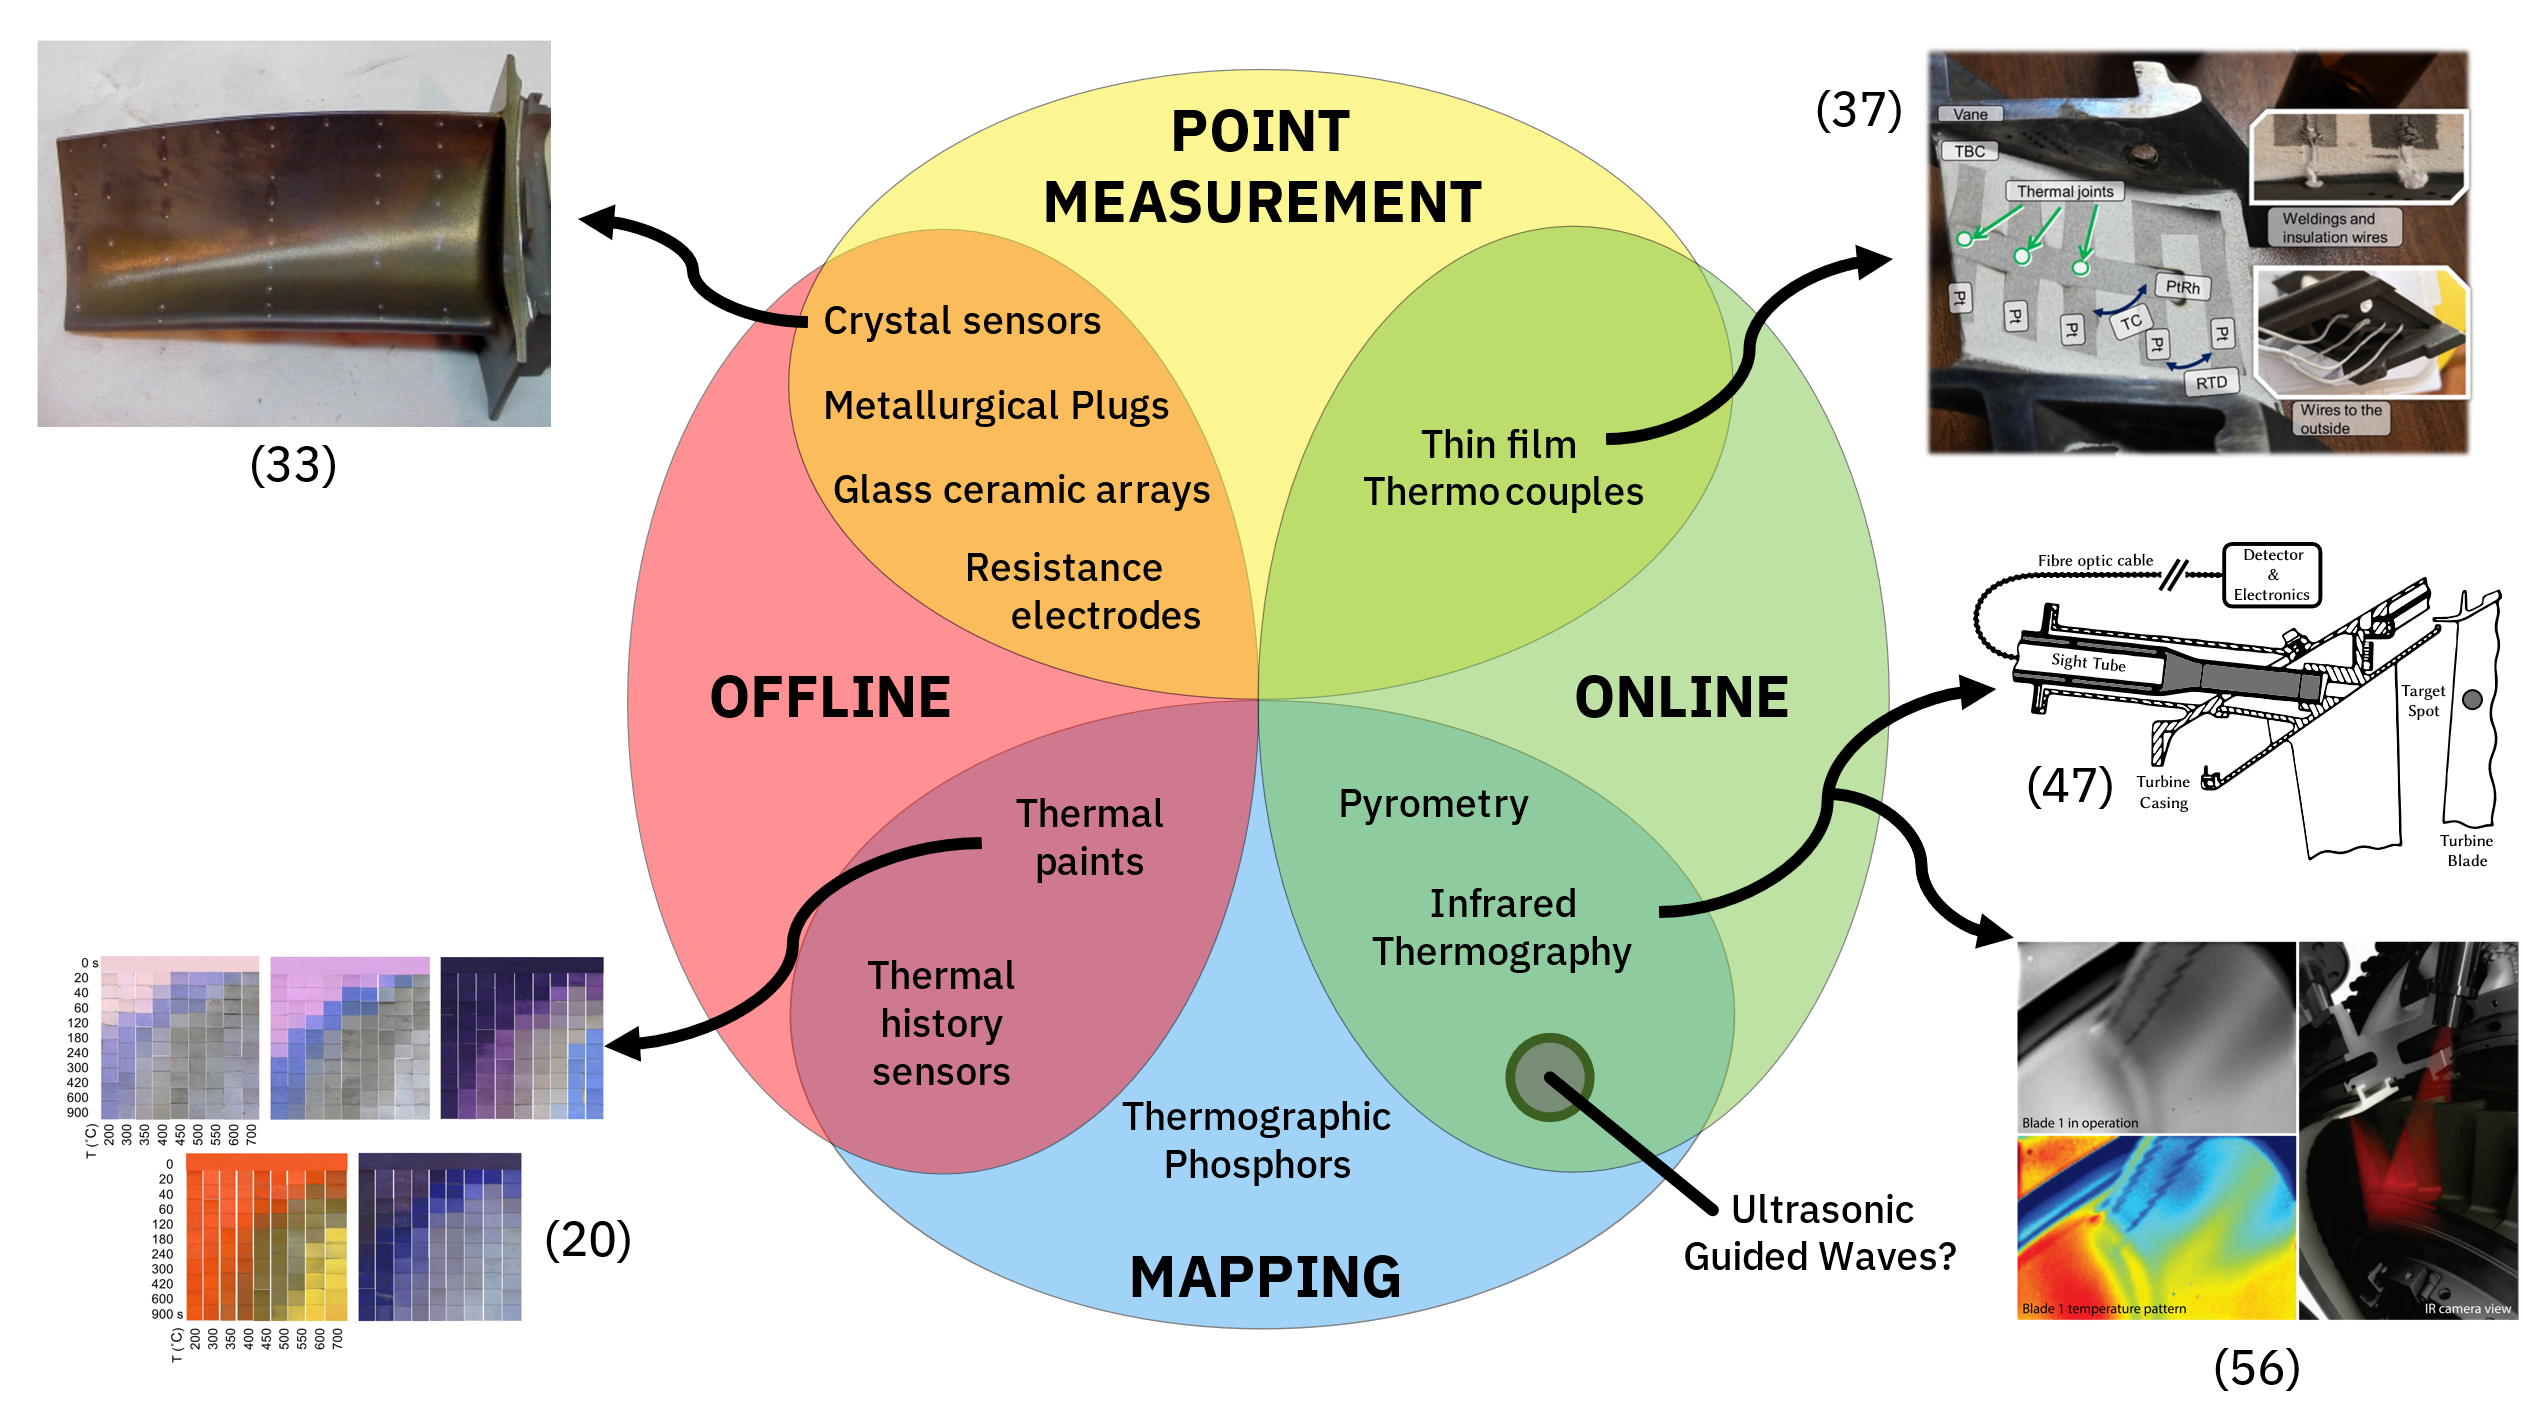
\includegraphics[width=\textwidth]{images/venndiagram.png}
\end{figure}
\end{frame}

%%%%%%%%%%%%%%%%

\section{Experimental study}
\begin{frame}{Experimental study}{Method}

\begin{itemize}
  \item The temperature sensitivities of the $S_0$, $A_1$, and $S_1$ modes have been verified experimentally by measuring a change in group velocity with temperature.
  \item Wedge transducers in a pitch-catch configuration are used to excite 1~mm, 2.5~mm, and 4~mm thick aluminium plates at 1 MHz.
  \item Time of flight is measured using a cross-correlation function.
  \item Group velocity is calculated using the distance between transducers.
\end{itemize}

  \begin{figure}[h]
    \centering
    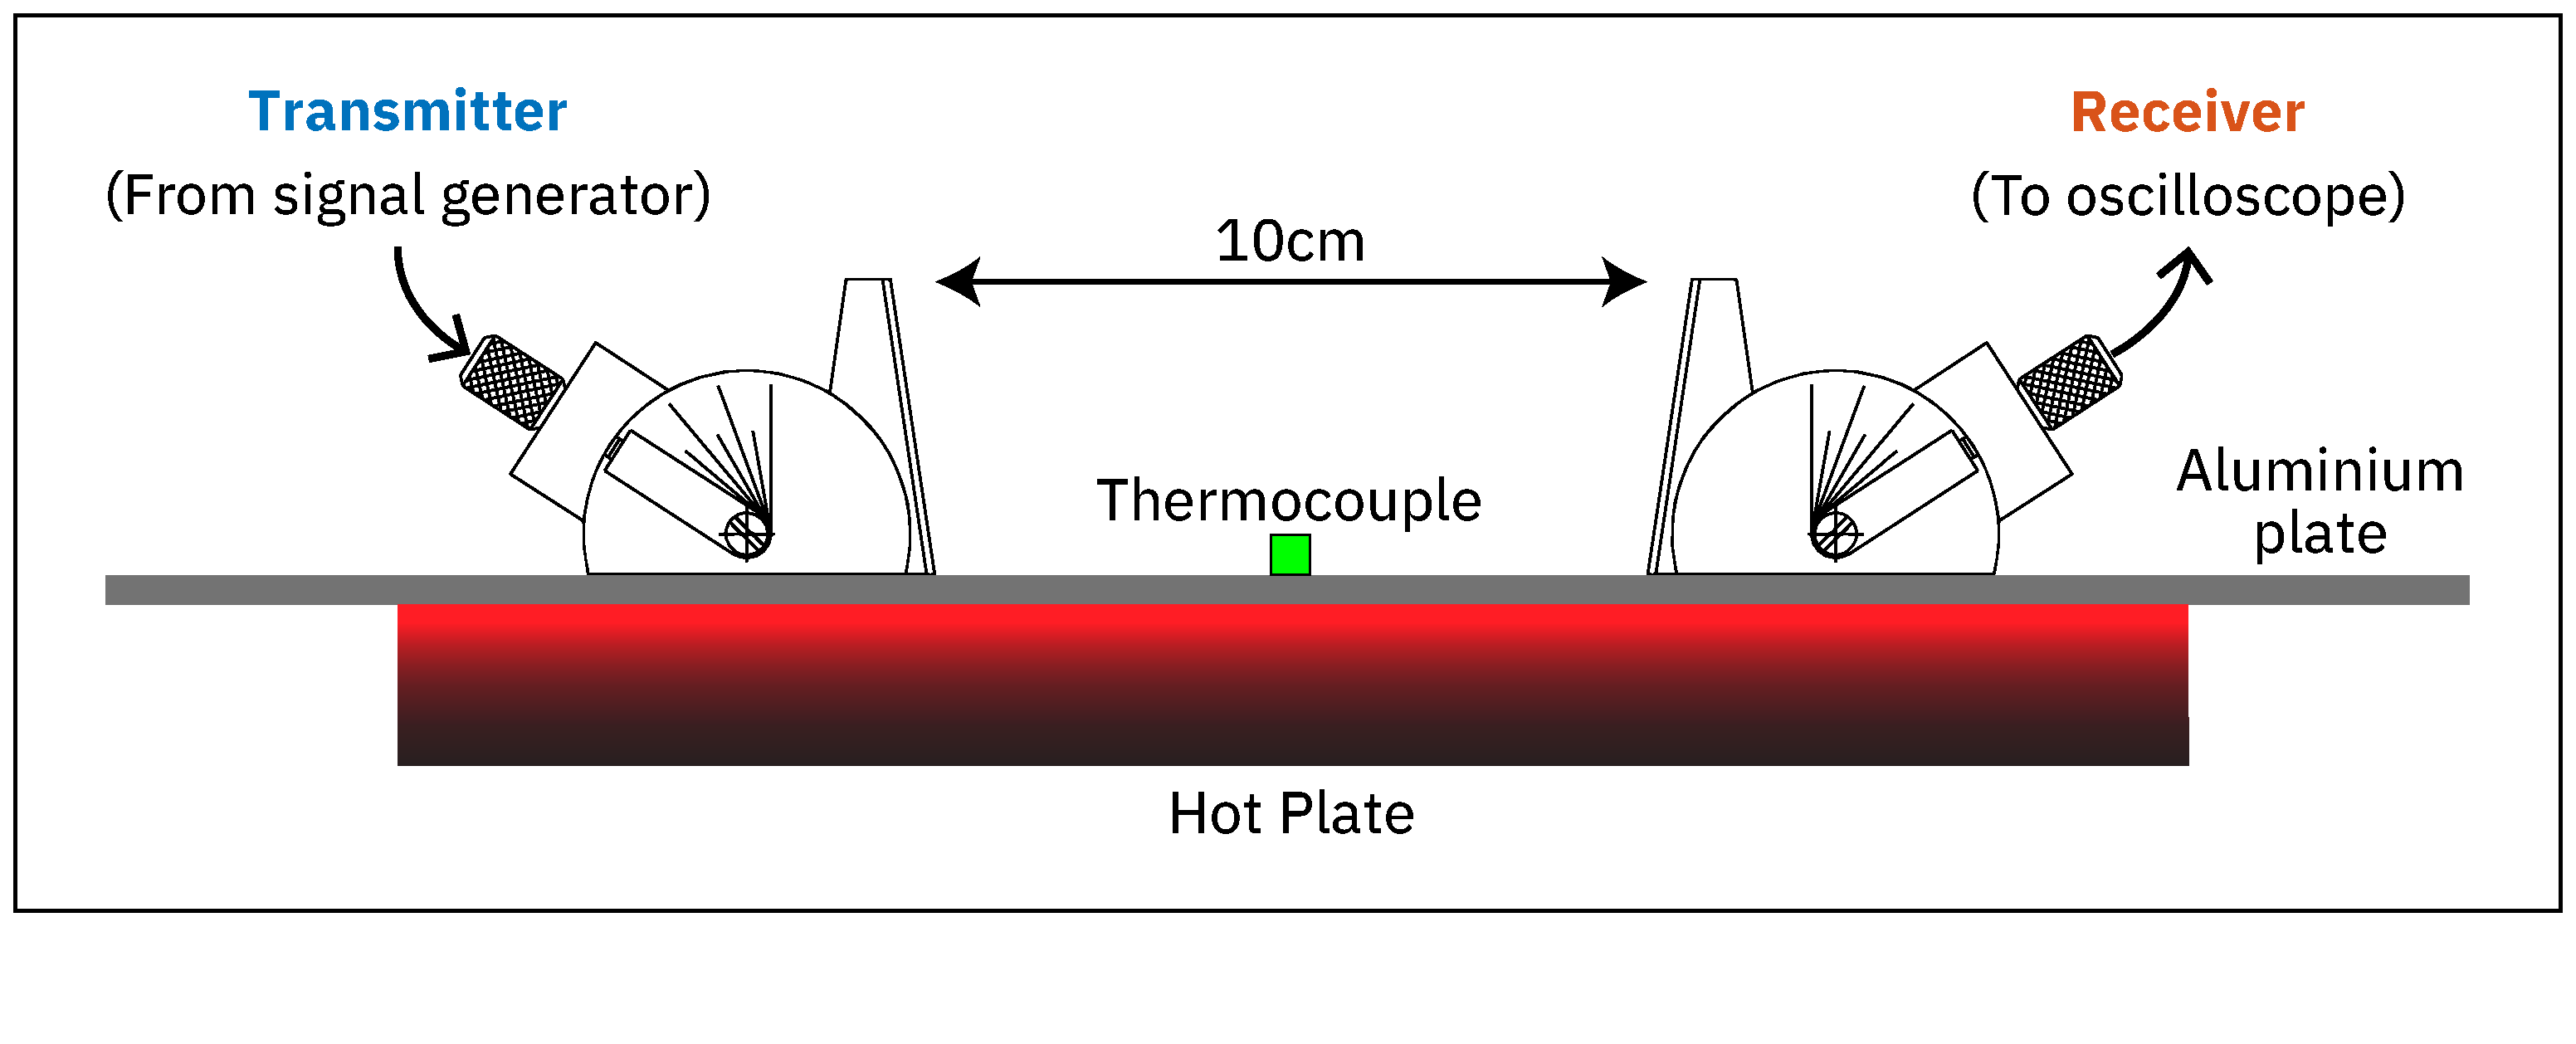
\includegraphics[width=0.75\textwidth]{images/testdiagramsimple.eps}
    \end{figure}
\end{frame}

%%%%%%%%%%%%%%%%

\begin{frame}{Experimental study}{Results}

  \begin{columns}
    \begin{column}{0.5\textwidth}
       \begin{center}
        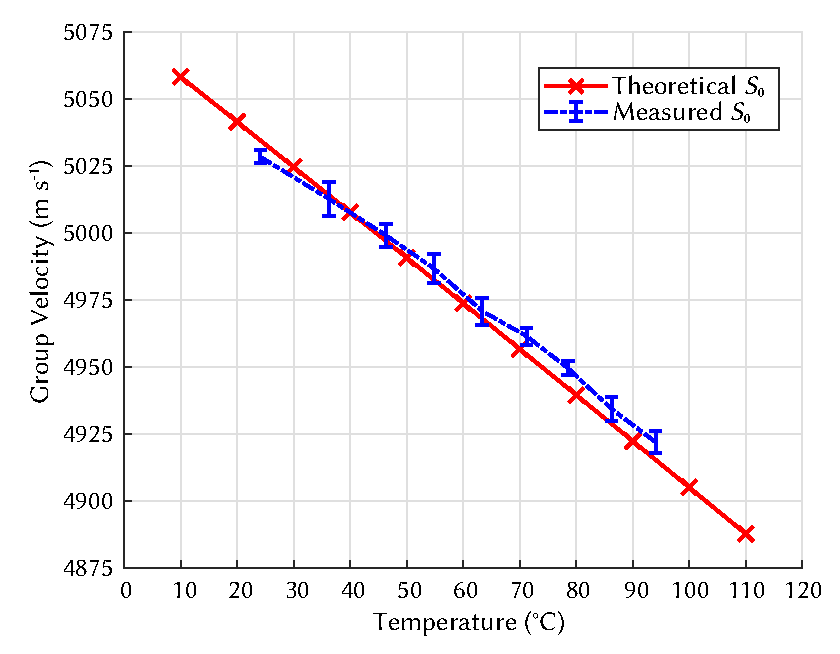
\includegraphics[width=\textwidth]{images/aluplatemeasured.eps}
       \end{center}
    \end{column}
    \begin{column}{0.5\textwidth}  %%<--- here
      \begin{center}
        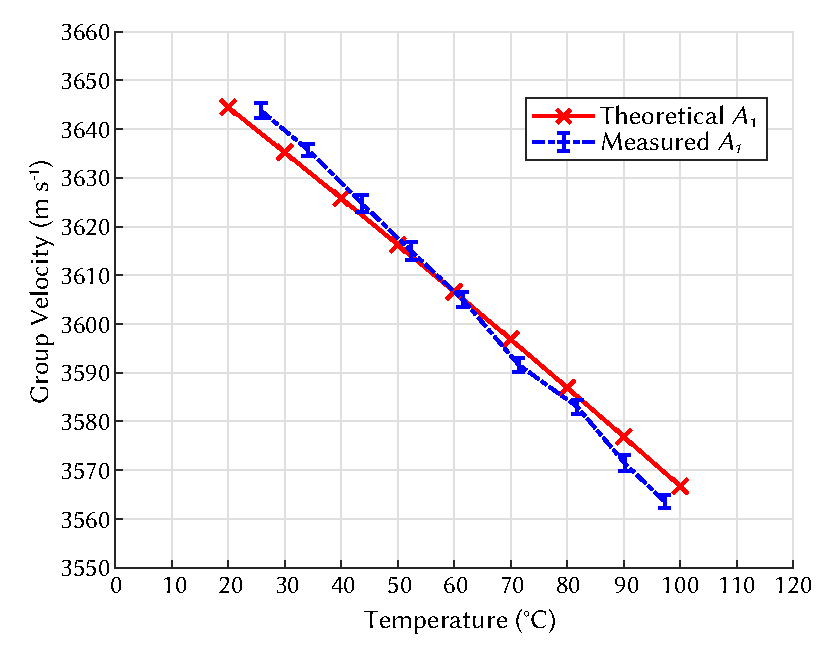
\includegraphics[width=0.7\textwidth]{images/a1moderesult.eps}
       \end{center}
       \begin{center}
        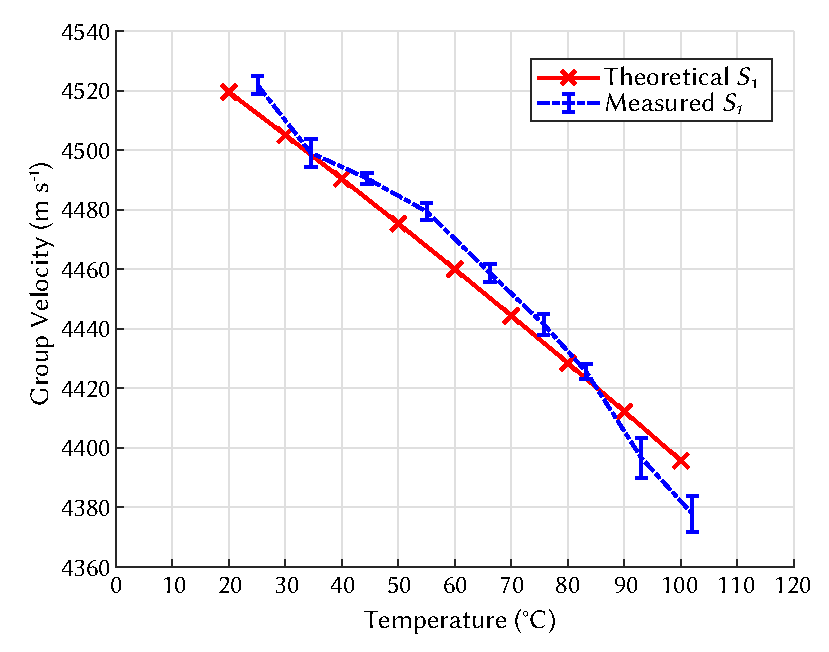
\includegraphics[width=0.7\textwidth]{images/s1moderesult.eps}
       \end{center}
    \end{column}
  \end{columns}
\end{frame}

%%%%%%%%%%%%%%%%

\section{COMSOL model}
\begin{frame}{COMSOL model}

\begin{itemize}
    \item Model initially developed to mimic experimental setup and verify experimental results.
    \item Group velocity of $S_0$ mode is comparable with theoretical/experimental results.
    \item Model will be used in the future to investigate the effect of cooling holes and TBCs on wave propagation. 
    \item A new model will be developed to investigate the suitability of a waveguide transducer system.  
\end{itemize}

\begin{center}
  \includegraphics[width=\textwidth]{images/comsoldiagram.png}
 \end{center}

\end{frame}

%%%%%%%%%%%%%%%%

\section{Future plans}
\begin{frame}{Future plans}
  \begin{itemize}
    \item The effect of plate holes on Lamb wave mode propagation will be investigated through simulation and experimentation.
    \item The ability to monitor temperature at a number of locations through the analysis of acoustic reflections will be explored.
    \item The effect of thermal barrier coatings (TBCs) on wave propagation will be investigated using COMSOL models.
    \item COMSOL simulations will be used to investigate the use of a new transducer configuration that can operate at high temperatures, mostly likely utilising wave guides and Hertzian contact points.
    \item Depending on the outcome of the previous COMSOL study and time constraints, a waveguide system will be tested experimentally.
\end{itemize}
\end{frame}

%%%%%%%%%%%%%%%%
\section{Gantt chart}
\begin{frame}{Gantt chart}
  \begin{figure}
    \centering
    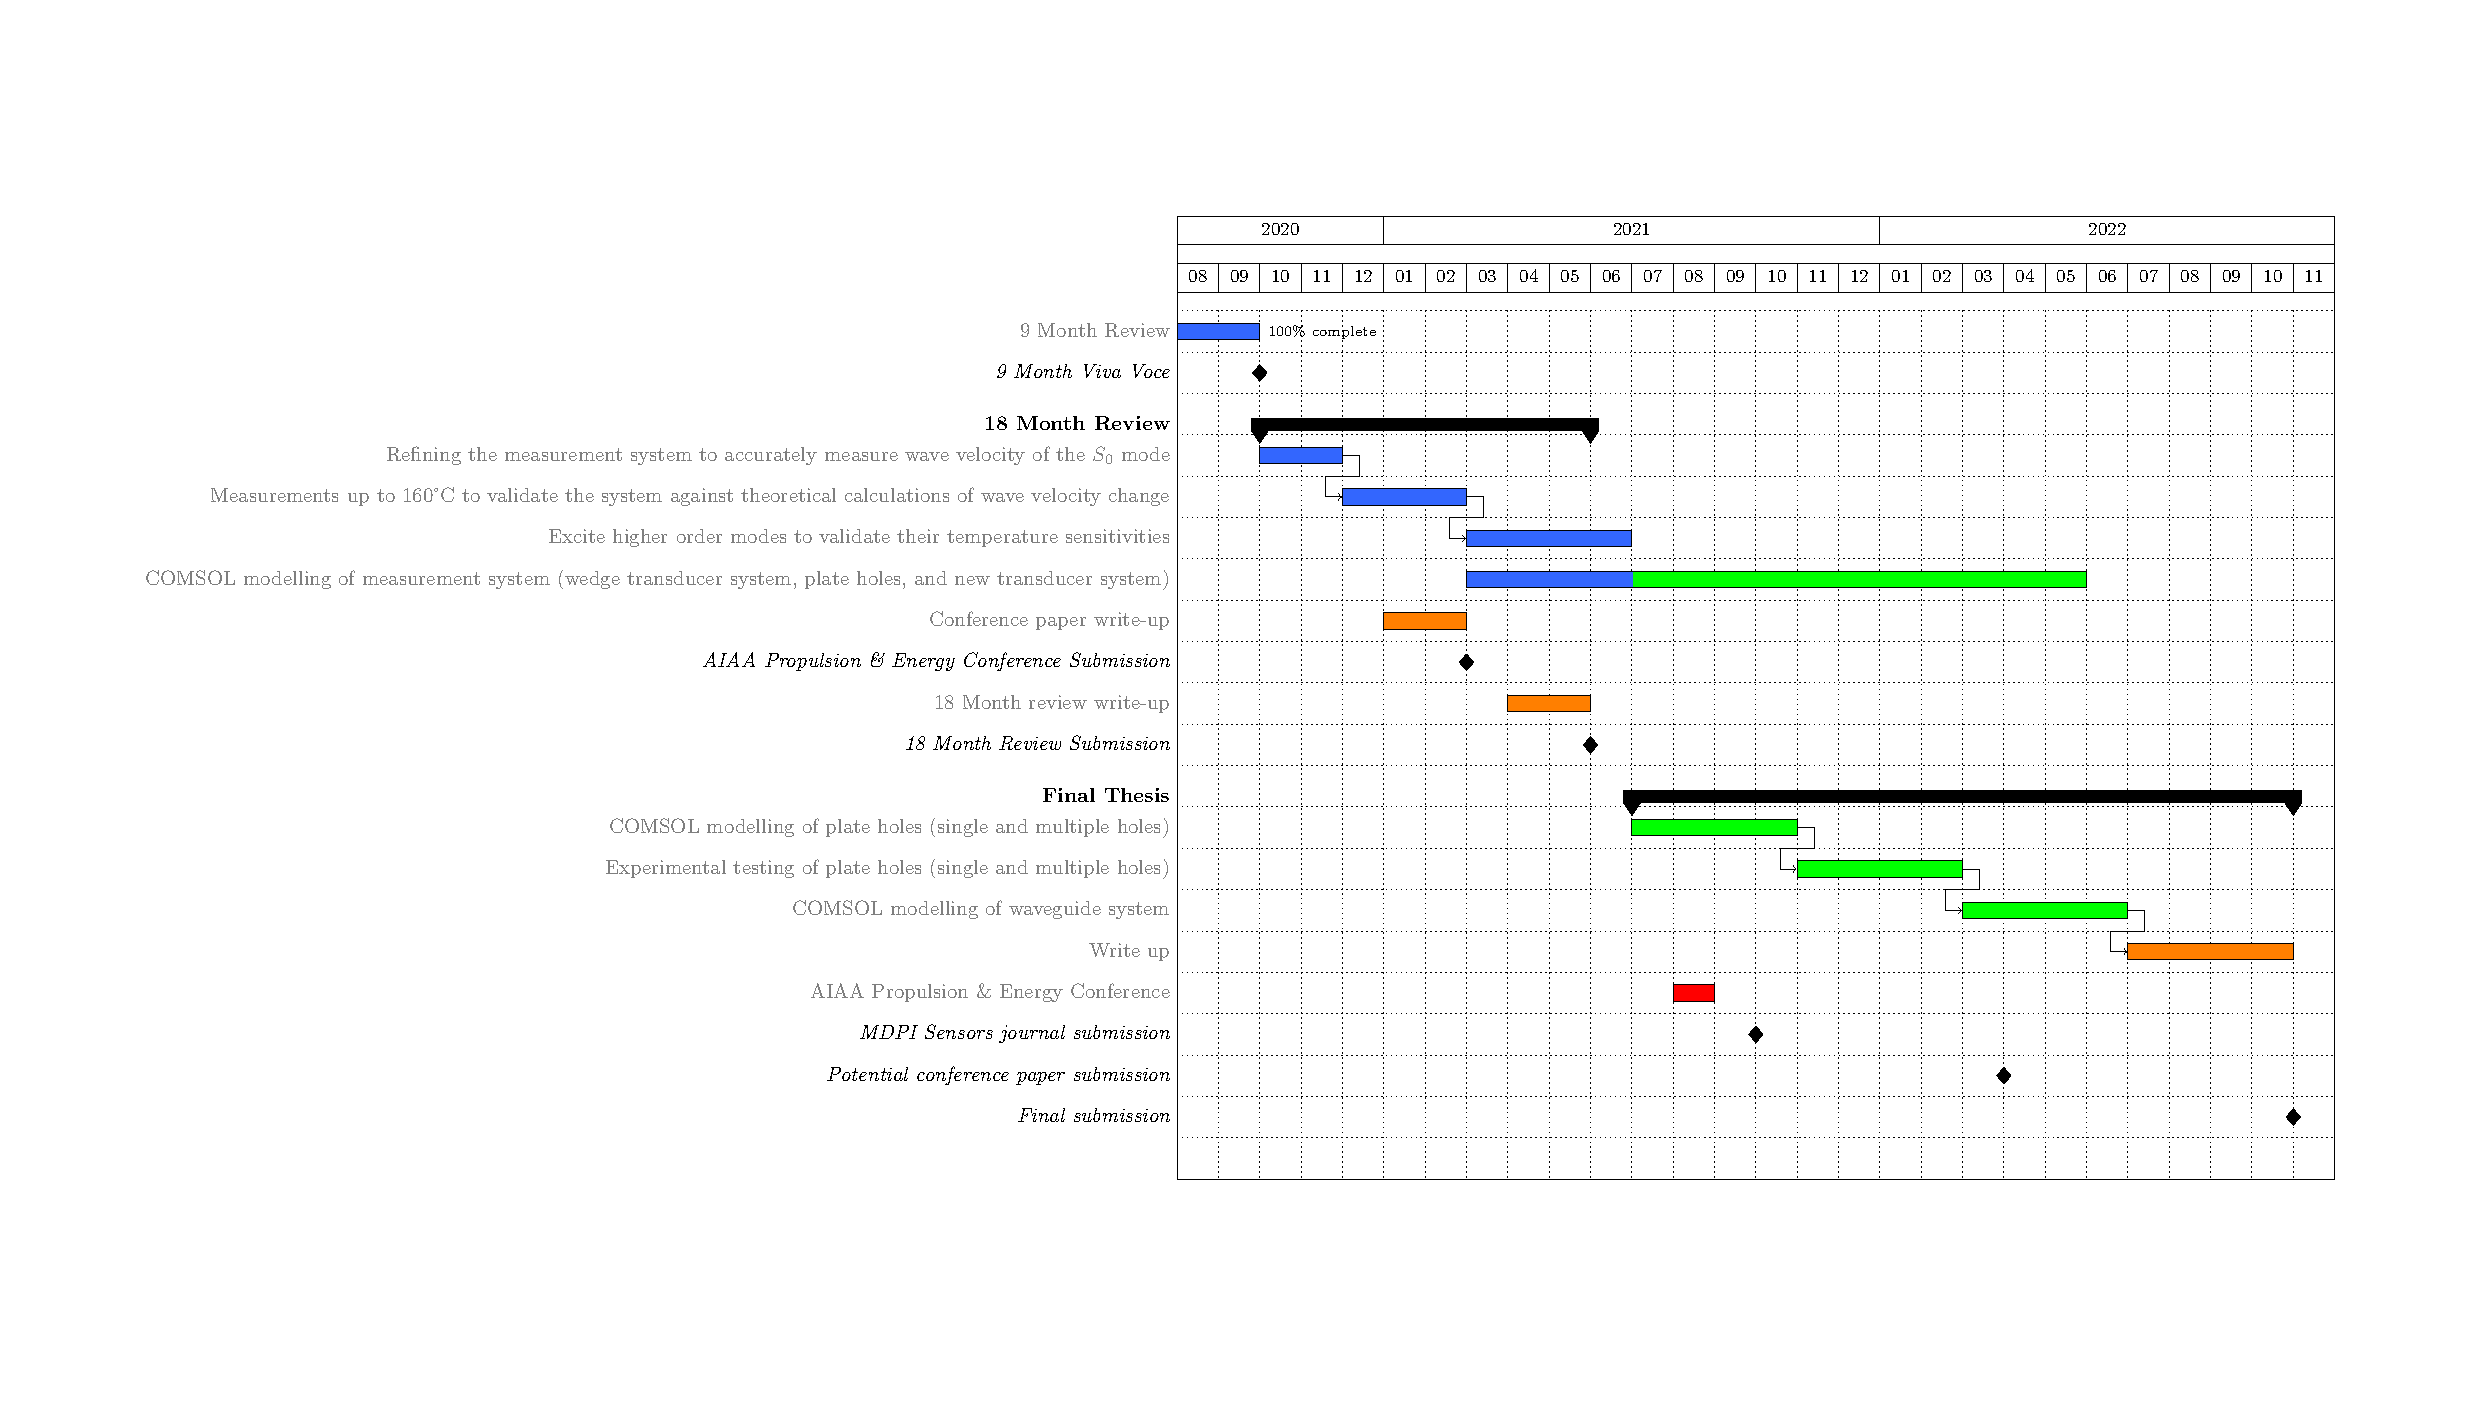
\includegraphics[width=\textwidth]{images/gantt.pdf}
  \end{figure}
\end{frame}

%%%%%%%%%%%%%%%%

{\wavesbg%
\begin{frame}[plain,noframenumbering]%
  \finalpage{Thank you for listening!}
\end{frame}}
%%%%%%%%%%%%%%%%

\end{document}
